\newpage
\section*{Appendix}

\section{AUC comparison}
\label{sec:appendix:auc}

\begin{table}[h!]
\caption{AUC scores under different noise levels for RCExplainer.}
\label{tab:appendix:auc_rcexplainer}
\centering
\resizebox{\columnwidth}{!}{
\begin{tabular}{ llllllll  }
 \toprule
Noise level &  0 & 0.05 & 0.1 & 0.15 & 0.2 & 0.25 & 0.3 \\
 \midrule
All (FN+FP+TN+TP) & 1.0000 & 0.9994 & 0.9981 & 0.9968 & 0.9960 & 0.9951 & 0.9945 \\
Original (TP+FP) & 0.9909 & 0.9512 & 0.8969 & 0.8475 & 0.8051 & 0.7622 & 0.7368 \\
False negatives (TP+FP+FN) & 0.9909 & 0.9503 & 0.8941 & 0.8429 & 0.7998 & 0.7560 & 0.7302 \\
Original and false negatives difference & 0.000\%& 0.091\%& 0.309\%& 0.546\%& 0.659\%& 0.811\%& 0.895\% \\
 \bottomrule
\end{tabular}}
\end{table}

\begin{table}[h!]
\caption{AUC scores under different noise levels for PGExplainer.}
\label{tab:appendix:auc_pgexplainer}
\centering
\resizebox{\columnwidth}{!}{
\begin{tabular}{ llllllll  }
 \toprule
Noise level &  0 & 0.05 & 0.1 & 0.15 & 0.2 & 0.25 & 0.3 \\
 \midrule
All (FN+FP+TN+TP) & 0.9996 & 0.9988 & 0.9974 & 0.9964 & 0.9945 & 0.9933 & 0.9926 \\
Original (TP+FP) & 0.9279 & 0.8810 & 0.8293 & 0.7846 & 0.7487 & 0.7179 & 0.6941 \\
False negatives (TP+FP+FN) & 0.9279 & 0.8800 & 0.8265 & 0.7809 & 0.7425 & 0.7105 & 0.6863 \\
Original and false negatives difference & 0.000\%& 0.112\%& 0.339\%& 0.479\%& 0.822\%& 1.022\%& 1.127\% \\
 \bottomrule
 \end{tabular}}
\end{table}


As concerns were raised about the specifics of the AUC computation and its effect, the AUC of different approaches are shown in Table \ref{tab:appendix:auc_rcexplainer} for RCExplainer and Table \ref{tab:appendix:auc_pgexplainer} for PGExplainer. These scores are computed on the Mutagenicity dataset using the provided pre-trained model for RCExplainer and PGExplainer, trained using the provided script and parameters. The effect is most notable under the highest noise levels, which causes $S'$ to differ the most from $S$. The original approach is positively biased for all explainers, but not equally and, therefore, affects the comparison. The effect is small enough that we chose to ignore it to retain the ability to compare to the original paper. 


\section{Hardware}
\label{appendix:hardware}
\begin{table}[h]
\centering
\caption{Hardware specifications of the machines used for training.}
\label{tab:appendix:hwspec}
\begin{tabular}{ll}
\toprule 
CPU    & Intel i9-9900 @ 3.10 GHz      \\
GPU    & NVIDIA GeForce RTX 2080 Ti   \\
Memory & 64 GB                        \\
\bottomrule
\end{tabular}
\end{table}

\section{MNISTSuperpixels GNN Training}
\label{appendix:GNN_training}
For the MNISTSuperpixels dataset, we deviated from the GNN architecture used by the original authors, as it had low performance. A high accuracy of the prediction model is important because it validates the counterfactuals produced by the explanation model. A poorly trained prediction model may have arbitrary explanations, even if the explanation model is correctly trained, and therefore does not have meaningful counterfactuals. A properly trained explanation model should allow for qualitative evaluation of the method.

By increasing the number of layers and hidden dimensions of the model, the larger GNN achieves a test-set score of 85\% accuracy, just short of the test-set score reached in \cite{dwivedi2020benchmarking}. This is shown in  Figure \ref{fig:MNIST_training_GNN}. Training for the baseline model was stopped early due to low performance.


\begin{figure}[!htbp]
    % \centering
    \centerline{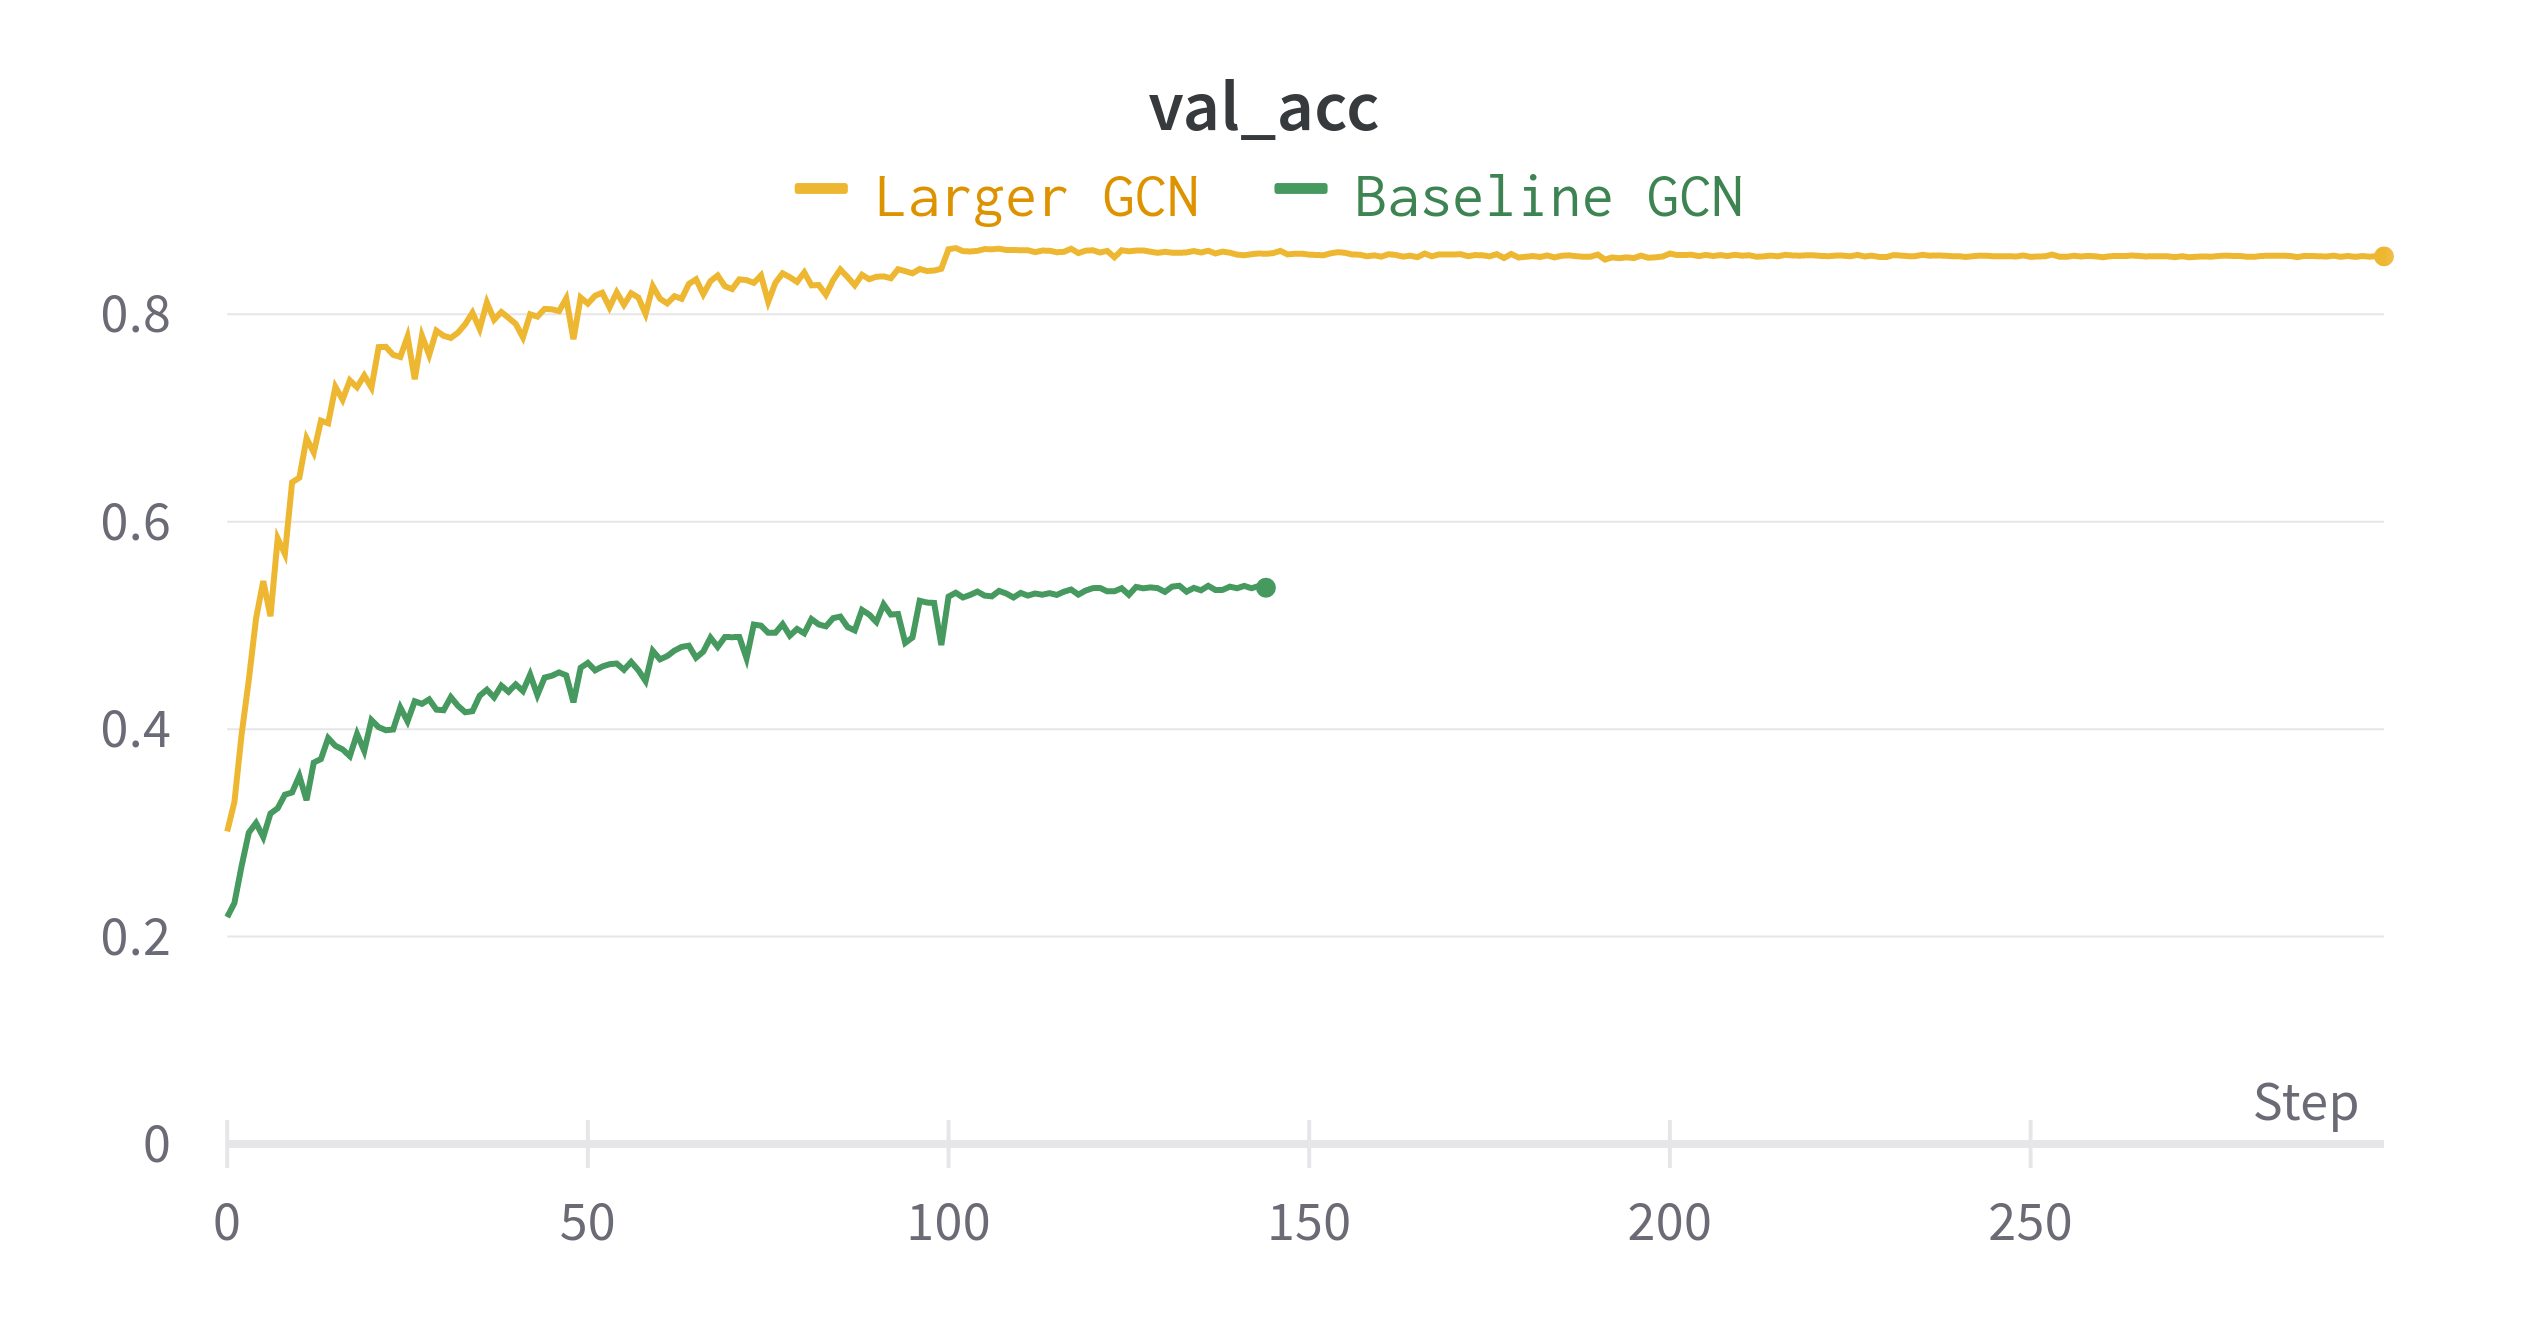
\includegraphics[width=.9\textwidth,trim={0 0 0 5cm},clip]{Images/MNIST_GCN.png}}
    \caption{Validation accuracy of GNN on MNISTSuperpixels dataset.}
    \label{fig:MNIST_training_GNN}
\end{figure}

\newpage
\section{MNISTSuperpixels Qualitative Results}
\begin{figure}[!htbp]
    % \centering
    \centerline{\includegraphics[width=1\textwidth]{Images/MNISTGrid_bigboy.png}}
    \caption{Node Explanations on MNISTSuperpixels dataset.}
    \label{fig:qual_MNIST}
\end{figure}

Figure \ref{fig:qual_MNIST} shows the qualitative results of the RCExplainer model on the MNISTSuperpixels dataset, using twelve randomly sampled graphs. The nodes overlayed on the images are the centroids of the superpixels of the input images, and the brighter their colour, the higher their probability of being included in the explanation of the model.

\noindent While the original authors mainly define the explanation to be a set of edges they also provide a definition for an explanation consisting of nodes, which we employed for this visualization. There, a node $n \in N$ has a weight $a_{n}$, defined as follows:
\begin{equation}
    a_{n} = \max_{i \in N}(\textbf{M}_{ni}),
\end{equation}
where $\textbf{M}$ is the matrix generated by the explanation network $f_{\theta}$. This means that the weight of a node corresponds to the probability of the edge with the highest probability of belonging to the explanation. Every node with a weight higher than $0.5$ is then considered to be part of the explanation of that graph.

\newpage

\section{Hyperparameter comparison} \label{appendix:hyperparameters}

\begin{figure}[h!]
    \centering
    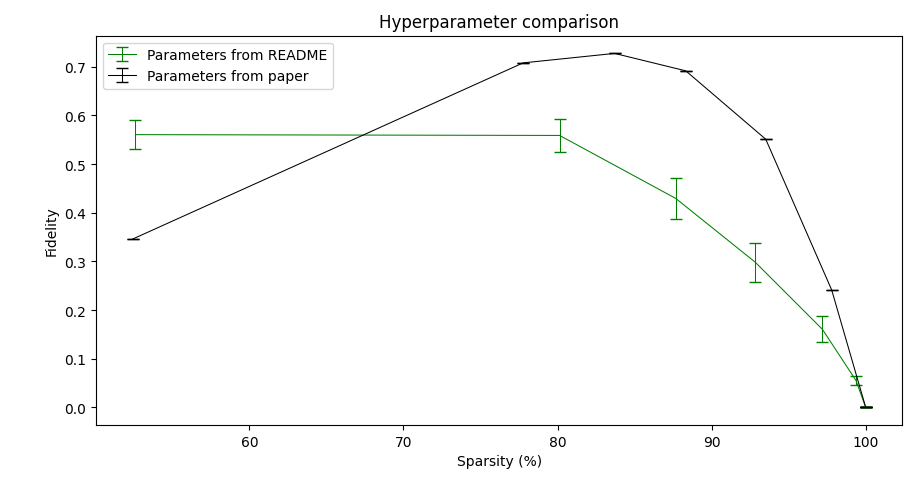
\includegraphics[width=\linewidth]{Images/fidelity_hyperparameters.png}
    \caption{Comparison between two explainer models on the metric \textit{fidelity} using a 100/100\% train-test split.}
\end{figure}

\begin{figure}[h!]
    \centering
    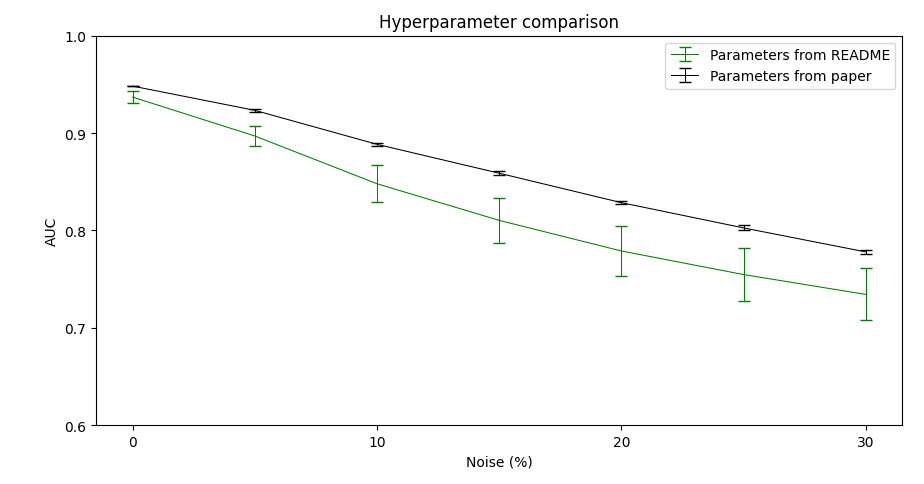
\includegraphics[width=\linewidth]{Images/noise_hyperparameters.png}
    \caption{Comparison between two explainer models on the metric \textit{robuustness} using a 100/100\% train-test split.}
\end{figure}

